\documentclass[journal,12pt,twocolumn]{IEEEtran}
\usepackage{setspace}
\usepackage{gensymb}
\singlespacing
\usepackage[cmex10]{amsmath}

\usepackage{amsthm}
\usepackage{hyperref}
\hypersetup{
    colorlinks=true,
    linkcolor=blue,
    filecolor=magenta,      
    urlcolor=cyan,
}

\urlstyle{same}
\usepackage{mathrsfs}
\usepackage{txfonts}
\usepackage{stfloats}
\usepackage{bm}
\usepackage{cite}
\usepackage{cases}
\usepackage{subfig}

\usepackage{longtable}
\usepackage{multirow}

\usepackage{enumitem}
\usepackage{mathtools}
\usepackage{steinmetz}
\usepackage{tikz}
\usepackage{circuitikz}
\usepackage{verbatim}
\usepackage{tfrupee}
\usepackage[breaklinks=true]{hyperref}
\usepackage{graphicx}
\usepackage{tkz-euclide}

\usetikzlibrary{calc,math}
\usepackage{listings}
    \usepackage{color}                                            %%
    \usepackage{array}                                            %%
    \usepackage{longtable}                                        %%
    \usepackage{calc}                                             %%
    \usepackage{multirow}                                         %%
    \usepackage{hhline}                                           %%
    \usepackage{ifthen}                                           %%
    \usepackage{lscape}     
\usepackage{multicol}
\usepackage{chngcntr}
\usepackage{mdframed}
\DeclareMathOperator*{\Res}{Res}

\renewcommand\thesection{\arabic{section}}
\renewcommand\thesubsection{\thesection.\arabic{subsection}}
\renewcommand\thesubsubsection{\thesubsection.\arabic{subsubsection}}

\renewcommand\thesectiondis{\arabic{section}}
\renewcommand\thesubsectiondis{\thesectiondis.\arabic{subsection}}
\renewcommand\thesubsubsectiondis{\thesubsectiondis.\arabic{subsubsection}}


\hyphenation{op-tical net-works semi-conduc-tor}
\def\inputGnumericTable{}                                 %%

\lstset{
%language=C,
frame=single, 
breaklines=true,
columns=fullflexible
}

\usepackage{chngcntr}
\counterwithin{figure}{section}

\title{AI5002}
\author{TUHIN DUTTA}
\date{January 2021}

\begin{document}
\newtheorem{theorem}{Theorem}[section]
\newtheorem{problem}{Problem}
\newtheorem{proposition}{Proposition}[section]
\newtheorem{lemma}{Lemma}[section]
\newtheorem{corollary}[theorem]{Corollary}
\newtheorem{example}{Example}[section]
\newtheorem{definition}[problem]{Definition}

\newcommand{\BEQA}{\begin{eqnarray}}
\newcommand{\EEQA}{\end{eqnarray}}
\newcommand{\define}{\stackrel{\triangle}{=}}
\bibliographystyle{IEEEtran}
\raggedbottom
\setlength{\parindent}{0pt}
\providecommand{\mbf}{\mathbf}
\providecommand{\pr}[1]{\ensuremath{\Pr\left(#1\right)}}
\providecommand{\qfunc}[1]{\ensuremath{Q\left(#1\right)}}
\providecommand{\sbrak}[1]{\ensuremath{{}\left[#1\right]}}
\providecommand{\lsbrak}[1]{\ensuremath{{}\left[#1\right.}}
\providecommand{\rsbrak}[1]{\ensuremath{{}\left.#1\right]}}
\providecommand{\brak}[1]{\ensuremath{\left(#1\right)}}
\providecommand{\lbrak}[1]{\ensuremath{\left(#1\right.}}
\providecommand{\rbrak}[1]{\ensuremath{\left.#1\right)}}
\providecommand{\cbrak}[1]{\ensuremath{\left\{#1\right\}}}
\providecommand{\lcbrak}[1]{\ensuremath{\left\{#1\right.}}
\providecommand{\rcbrak}[1]{\ensuremath{\left.#1\right\}}}
\theoremstyle{remark}
\newtheorem{rem}{Remark}
\newcommand{\sgn}{\mathop{\mathrm{sgn}}}

\providecommand{\res}[1]{\Res\displaylimits_{#1}} 

%\providecommand{\norm}[1]{\lVert#1\rVert}
\providecommand{\mtx}[1]{\mathbf{#1}}
\providecommand{\fourier}{\overset{\mathcal{F}}{ \rightleftharpoons}}
%\providecommand{\hilbert}{\overset{\mathcal{H}}{ \rightleftharpoons}}
\providecommand{\system}{\overset{\mathcal{H}}{ \longleftrightarrow}}
	%\newcommand{\solution}[2]{\textbf{Solution:}{#1}}
\newcommand{\solution}{\noindent \textbf{Solution: }}
\newcommand{\cosec}{\,\text{cosec}\,}
\providecommand{\dec}[2]{\ensuremath{\overset{#1}{\underset{#2}{\gtrless}}}}
\newcommand{\myvec}[1]{\ensuremath{\begin{pmatrix}#1\end{pmatrix}}}
\newcommand{\mydet}[1]{\ensuremath{\begin{vmatrix}#1\end{vmatrix}}}
\numberwithin{equation}{subsection}
\makeatletter
\@addtoreset{figure}{problem}
\makeatother
\let\StandardTheFigure\thefigure
\let\vec\mathbf
\renewcommand{\thefigure}{\theproblem}
\def\putbox#1#2#3{\makebox[0in][l]{\makebox[#1][l]{}\raisebox{\baselineskip}[0in][0in]{\raisebox{#2}[0in][0in]{#3}}}}
     \def\rightbox#1{\makebox[0in][r]{#1}}
     \def\centbox#1{\makebox[0in]{#1}}
     \def\topbox#1{\raisebox{-\baselineskip}[0in][0in]{#1}}
     \def\midbox#1{\raisebox{-0.5\baselineskip}[0in][0in]{#1}}
\vspace{3cm}
\title{AI5002 - Assignment 4}
\author{Tuhin Dutta\\ ai21mtech02002}
\maketitle
\newpage
\bigskip
\renewcommand{\thefigure}{\theenumi}
\renewcommand{\thetable}{\theenumi}
\begin{mdframed}
Download code and LaTeX from below hyperlinks\\
1. \href{https://github.com/Tauhait/AI5002/blob/main/Assignment-4/Codes/Binomial\_3\_3.py}{Codes/Binomial\_3\_3.py}


2. \href{https://github.com/Tauhait/AI5002/tree/main/Assignment-4/LaTeX}{LaTeX}
\end{mdframed}
\subsection*{\boldsymbol{Problem\ 3.3}}
\begin{flushleft}Suppose X has binomial distribution.\\ Show that X = 3 is the most likely outcome.\\ (Hint: P\ (X=3) is the maximum among all P\ (\mathop{x_i}),\\\mathop{x_i} = 0, 1, 2, 3, 4, 5, 6)\end{flushleft}

\subsection*{\boldsymbol{Solution}}\\
We can write,
\begin{align*}X \sim B\ (n, p)\end{align*}
\begin{flushalign}\\where n is the number of independent trials,\\ p is the probability of success for each trial and\\ q is the probability of failure = 1 - p for each trial.\end{flushalign}\\

%Let's take n = 6,  p = \dfrac{1}{2}\ and\ q = \dfrac{1}{2}.\\

Then, 
\begin{align}
P\ (X = x) = \binom{\ n\ }{\ x\ }.\ q^{\ n-x\ }.\ p^{\ x\ }
\end{align}
Putting value of x = 3 and assuming p = $\dfrac{1}{2}$ while q = 1 - p = $\dfrac{1}{2}$ in (0.0.1), we get\\
\begin{align}
P\ (X = 3) = \binom{\ n\ }{\ 3\ }.\ \Big(\dfrac{1}{2}\Big)^{\ n-3\ }.\ \Big({\dfrac{1}{2}}\Big)^{\ 3\ }
\end{align}
\begin{align}
P\ (X = 3) = \binom{n}{3}.\ \Big(\dfrac{1}{2}\Big)^{\ n\ }
\end{align}\\

From (0.0.3) we can see that for P (X = 3) to be maximum the term $\mathop{\binom{\ n\ }{\ 3\ }}$ should be maximum. \\

From combinatorics we know for the term $\mathop{\binom{\ n\ }{\ 3\ }}$ to be maximum, n value should be  = 3 * 2 = 6.\\

For all given values of \begin{align*}\mathop{x_i} = \Big( 0, 1, 2, 3, 4, 5, 6 \Big)\end{align*} we find the P (X = \mathop{x_i}).\\

\begin{flushleft}For\ \mathop{x_i\ =\ 0},\end{flushleft}
\begin{align}P\ (X = 0) = \binom{6}{0}.\ \Big(\dfrac{1}{2}\Big)^{\ 6\ } = \dfrac{1}{64} = P\ (X = 6)\end{align}\\

\begin{flushleft}For\ \mathop{x_i\ =\ 1},\end{flushleft}
\begin{align}P\ (X = 1) = \binom{6}{1}.\ \Big(\dfrac{1}{2}\Big)^{\ 6\ } = \dfrac{6}{64} = P\ (X = 5)\end{align}\\

\begin{flushleft}For\ \mathop{x_i\ =\ 2},\end{flushleft}
\begin{align}P\ (X = 2) = \binom{6}{2}.\ \Big(\dfrac{1}{2}\Big)^{\ 6\ } = \dfrac{15}{64} = P\ (X = 4)\end{align}\\

\begin{flushleft}For\ \mathop{x_i\ =\ 3},\end{flushleft}
\begin{align}P\ (X = 3) = \binom{6}{3}.\ \Big(\dfrac{1}{2}\Big)^{\ 6\ } = \dfrac{20}{64} = 0.3125\end{align}
\\
\begin{flushleft}Comparing (0.0.4) through (0.0.7), we see X = 3 (0.0.7) to be the most likely event.\end{flushleft}

\begin{figure}[h!]
    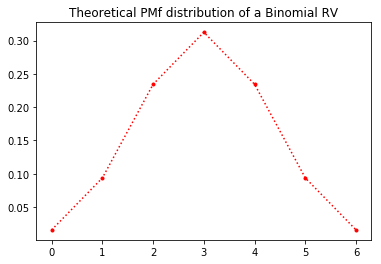
\includegraphics[width=8cm]{Assignment-4/Codes/Figures/theo_pmf.png}
    \caption*{Fig 1.1: Theoretical PMf plot}
\end{figure}
\begin{figure}[h!]
    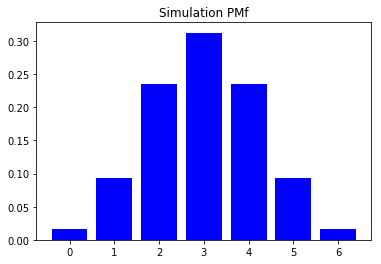
\includegraphics[width=8cm]{Assignment-4/Codes/Figures/sim_pmf.png}
    \caption*{Fig 1.2: Simulation plot of PMf}
\end{figure}
\begin{figure}[h!]
    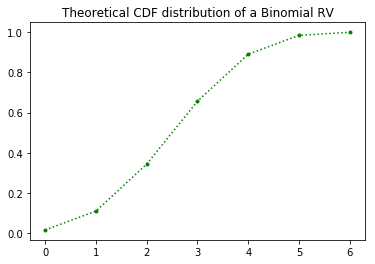
\includegraphics[width=8cm]{Assignment-4/Codes/Figures/theo_cdf.png}
    \caption*{Fig 1.3: Theoretical CDF plot}
\end{figure}
\begin{figure}[h!]
    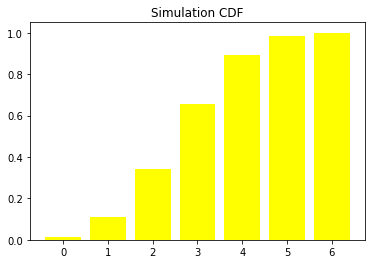
\includegraphics[width=8cm]{Assignment-4/Codes/Figures/sim_cdf.png}
    \caption*{Fig 1.4: Simulation plot of CDF}
\end{figure}
\end{document}
